\documentclass[../main.tex]{subfiles}
\chapter{Simulation}
\label{c:simulation}

\begin{figure}
	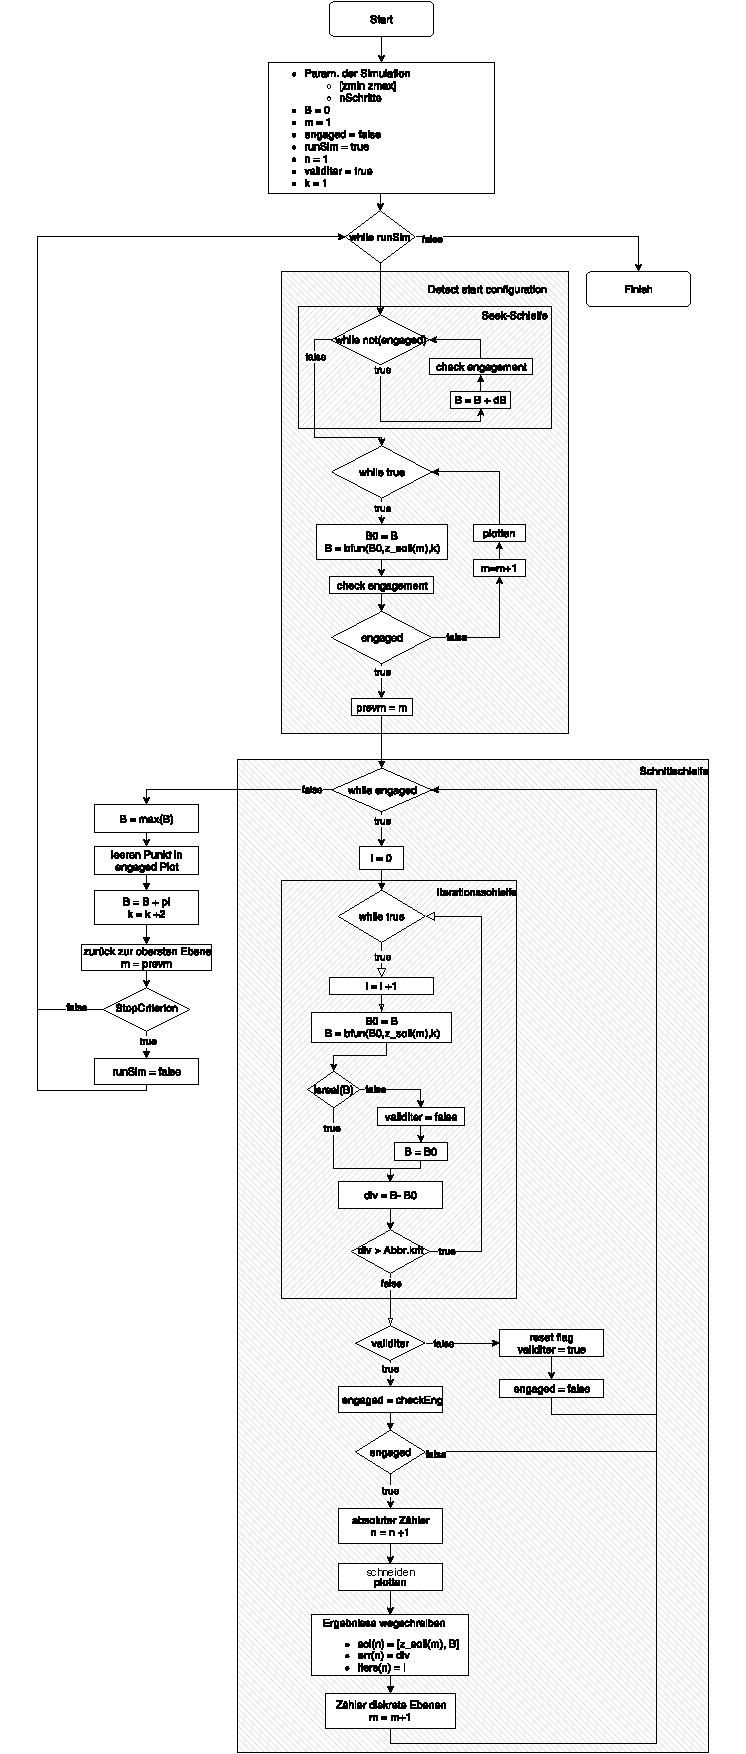
\includegraphics[scale=0.75]{vf1-flowchart}
	\caption{Flussbild der Simulationsschleife}
	\label{fig:flowchart}
\end{figure}

Abbildung \ref{fig:flowchart} zeigt das Flussbild der Simulation.
Der Ablauf der Simulation ist unterteilt in die Abschnitte Findung der Startkonfiguration, Durchführung der Schnitte mit den Lösungsiterationen, Erkennung des Schnittendes sowie Nachbereitung des Schnittes und schließlich Abschluss der Simulation.
Neben der Ausführung des Simulationscodes sollte der Status der Berechnung in Form von grafischen Ausgaben dargestellt werden.
Das Plotten von Daten in Echtzeit ist in \matlab schwierig zu realisieren, vor allem bei dreidimensionalen Datensätzen.
Die standardmäßig zur Verfügung gestellten Routinen sind nicht gut optimiert für eine schnelle Ausführungszeit und es ist notorisch schwierig \matlab Code multithread-fähig zu gestalten.
Die Lösungsansätze, um trotz dieser Herausforderungen die für die grafische Ausgabe beanspruchte Rechenzeit effizient zu nutzen und die Simulation möglichst geringfügig zu belasten, wird ebenfalls besprochen.

Die einzelnen Prozessschritte der Simulation werden im Folgenden mit Ausschnitten aus dem Code erläutert.
Der gesamte Code kann gefunden werden in dem GitHub Repository:\\
\centerline{\url{https://github.com/ChrisSchuster/ba}}
Dieses Repository enthält Dependecies von dem Repository:\\
\centerline{\url{https://github.com/ChrisSchuster/matlab-utils}}

\section{Vorbereitung der Simulation}
Im Codeausschnitt \ref{code:setup} wird gezeigt, wie zu Beginn der Simulation die Simulationssteuerungsparameter eingelesen werden.
Dabei werden zunächst die Eingabedaten des betrachteten Falles festgelegt.
Mit den folgenden Parametern kann definiert werden, wie dieser Fall gestaltet ist:
\begin{itemize}
	\item Zähnezahl des Zahnrades
	\item Modul des Zahnrades
	\item Geometrie des  Werkzeuges (Durchmesser, Kopf- und Fußhöhe)
\end{itemize}
Aus diesen Parametern können weitere Startbedingungen ermittelt werden.
So ist die Startposition des Werkzeugs und den daraus folgenden Positionen der Maschinenkomponenten zu berechnen, wie sie in Abschnitt \ref{c:maschkomppos} besprochen wurden.
Die Position der X-Achse der Maschine wird berechnet über den Achsabstand des gedachten Schneckengetriebes nach \cite[Gleichung 23.4]{Matek2017}:
\begin{equation*}
	a = \frac{d_{s1}+d_{s2}}{2}
\end{equation*}
\begin{eqdscr}{$d_{s1}$, $d_{s2}$}
	\item[$a$] Achsabstand
	\item[$d_{s1}$, $d_{s2}$] Teilkreisdurchmesser von Schneckenrad und Schnecke
\end{eqdscr}
\begin{minipage}{\textwidth}
Der Teilkreisdurchmesser des Schneckenrades wird berechnet nach \cite{Matek2017}:
\begin{equation*}
	d_{s1} = m \cdot z
\end{equation*}
\begin{eqdscr}{$m$}
	\item[$m$] Modul
	\item[$z$] Zähnezahl des Werkstückes
\end{eqdscr}
\end{minipage}
\lstinputlisting[caption = {Bedatung der Maschinenparameter}, linerange=4-32,firstnumber=4, label={code:setup}]{../ba/methods/vf1/vf1.m}

Der Vorschubfaktor der X-Achse $\feed{X}{\wz}$ ist im betrachteten Fall null, sie verändert also ihre Position ausgehend von der Startposition im Verlauf der Simulation nicht.

Für den Startwert der Y-Achse müssen die Größen $y$, Achsverschiebung im Ausgang, und $\yshift$ festgelegt werden.
Ebenso ist für den Achsvorschub der Y-Achse $\feed{Y}{\wz}$ ein Wert einzugeben.
Diese Größen sind im betrachteten Fall null.
Die Y-Achse verändert im betrachteten Fall ihre Position ausgehend von ihrem Startwert nicht.

Danach wird die Werkzeuggeometrie erzeugt.
Wie in Kapitel \ref{c:werkzeugkinematik} erläutert, wird die Geometrie des Werkzeuges in Zylinderkoordinaten beschrieben.
Dabei wird im aktuellen Stand das Bezugsprofil durch vier Eckpunkte dargestellt, deren Koordinaten mit einem Algorithmus von \scherbarth berechnet werden.
Da eine Zahnstange als Zahnrad mit unendlich großer Zähnezahl verstanden werden kann, haben ihre Zähne gerade Flanken \cite[Kap. 3]{Widmer1981}.
Eine Annäherung der Zahnstange mit vier Punkten ist deswegen zweckmäßig, obwohl Verrundungen am Zahnkopf damit noch nicht dargestellt werden können.

\lstinputlisting[caption = {Aufsetzen der Ausgangsdaten der Simulation}, linerange=35-74,firstnumber=35,label={code:startdata}]{../ba/methods/vf1/vf1.m}

Der Codeausschnitt \ref{code:startdata} zeigt, wie die Daten von Werkzeug und Werkstück in der Ausgangssituation erzeugt werden.
Das Werkzeug wird als Array aus Polyshape Objekten abgelegt.
Dazu werden zunächst eine Menge diskreter Eckpunkte auf einem Kreis mit definierbarem Durchmesser erzeugt.
Die Menge der Eckpunkte richtet sich an der Menge der geforderten diskreten Ebenen.
So soll sicher gestellt werden, dass sich die auf der Werkstückoberflächen liegenden Vertices zu gleichschenkligen Dreiecken vernetzen lassen.
Aus den Eckpunkten wird dann ein Polyshape Objekt erzeugt.
Dieses wird entsprechend der Anzahl der geforderten Ebenen in ein Array repliziert.
So entsteht ein individuelles Polyshape Objekt für jede geforderte Ebene.
Auch wird ein Vektor erzeugt, der gleich strukturiert ist und die z-Koordinaten der entsprechenden Ebene enthält.
Um mitverfolgen zu können, auf welche Weise ein Vertice einer Schnittgeomtrie entstanden ist, wird bei jeder Schnittoperation zu jedem Vertice ein entsprechender Wert zurückgegeben.
Diese Klassifikation wird für jede Schnittgeomtrie in einem Vektor gespeichert, der ebenfalls zu einem Array repliziert werden muss.

Die Simulation beginnt mit einem Ebenenindex $m$ von eins.
Es wird zunächst davon ausgegangen, dass die erste Ebene des Werkstücks geschnitten wird.
Vor jedem Schnitt wird die oberste Ebene ermittelt, die eine valide Schnittkonfiguration hervorbringt.
Wie diese Erkennung funktioniert wird in Abschnitt \ref{c:startkonfig} erläutert.

\section[Startkonfiguration]{Findung der Startkonfiguration}
\label{c:startkonfig}
Der erste Schritt zur Findung der Startkonfiguration bei jeder Werkzeugumdrehung ist die Suche nach einer Werkzeugkonfiguration bei welcher Kontakt zwischen Werkzeug und Werkstück auftritt.
Dieser Vorgang wird als Seeken, eine deutsche Form des englischen Wortes für ,,Suchen'', bezeichnet.
Dabei wird das Werkzeug im freien Raum rotiert bis Kontakt auftritt.
Im Anschluss wird eine valide Schnittkonfiguration gesucht.

Eine valide Schnittkonfiguration tritt auf, wenn die auf eine diskrete Ebene des Werkstücks projizierte Geometrie der Schneide Überdeckung mit der Werkstückgeometrie hat.
Bei der vorliegenden Simulation ist das Werkstück entlang seiner Ausdehnung in z-Richtung in diskrete Ebenen unterteilt, welche das Werkzeug auf der jeweiligen Höhe in $z$ schneiden.
Die dabei entstandene Verschneidungsgeometrie des Werkstücks mit der Ebene ist eine zweidimensionale Geometrie.
Diese Geometrie ist ein Polygon, welches mit der Menge diskreter Punkte beschrieben wird, welche die Ecken des Polygons bilden.
Die Beschreibung von Werkstück und Werkzeug als Polygone wird in Abschnitt \ref{c:schnitte} im Detail beschrieben.

Seeken geschieht in der Seek-Schleife, die im Flussdiagrams in Abbildung \ref{fig:flowchart} eingetragen ist.
Dabei wird der Winkel des Werkzeugs ausgehend vom seiner Startkonfiguration mit einer bedatbaren Schrittweite inkrementiert, bis ein Punkt der Werkzeugschneide in der Hüllgeometrie des Werkstücks liegt.
Befindet sich ein Punkt des Werkzeugs in Hüllgeometrie des Werkstücks ist das Werkzeug ,,engaged'', angelehnt an das englische Wort für ,,eingerastet''; die Schneide befindet sich im Eingriff.

Die Hüllgeomtrie des Werkstücks entspricht der Form des Rohmaterials und ist somit ein Zylinder mit dem Durchmesser und der Höhe des Werkstücks.
Die Lage des Werkstücks entlang der z-Achse des Bearbeitungstischkoordinatensystems ist definierbar.

\lstinputlisting[caption = {Funktion zur Prüfung des Engagements}, linerange={1-1,7-19}]{../ba/fun/checkEngagement/checkEng.m}

Engagement wird in der Funktion \code{checkEng} durch Vergleich der Position der Schneidenecken mit der Ausdehnung des Werkstücks erkannt.
Dabei ist es geschickt die Position der Schneidenecken in Zylinkerkoordinaten zu beschreiben.
Vergleichbar zu den deckungsgleichen kartesischen und zylindrischen Koordinatensystemen des Werkzeugs, kann auch das Werkstück in kartesischen und zylindrischen Koordinatensystemen beschrieben werden.
Dieses Zylinderkoordinatensystem ist im Ursprung des kartesischen Werkzeugkoordinatensystems aufgespannt.
Die Koordinaten eines Punktes werden durch einen Winkel, einen Radius und eine Höhe in z-Richtung beschrieben.

Damit ein Punkt des Werkzeugs als engaged gilt, müssen zwei Bedingungen erfüllt sein:
Zum einen muss der Abstand des Punktes zum Ursprung kleiner als der Radius des Werkstücks sein.
Zum anderen muss der Wert seiner z-Koordinate im Intervall der Ausdehnung des Werkstücks liegen.
Der Winkel des Punktes spielt zur Engagementerkennung keine Rolle.
Der Abstand $d$ des Punktes zum Ursprung wird als euklidische Norm berechnet nach \cite{mwVecnorm}:
\begin{equation*}
	d = \|v\| = \sqrt{\sum_{k=1}^{N} \|v_k\|^2}
\end{equation*}
Die Funktion gibt als logischen Wert zurück, ob der Werkzeugpunkt engaged ist oder nicht.

\begin{figure}
	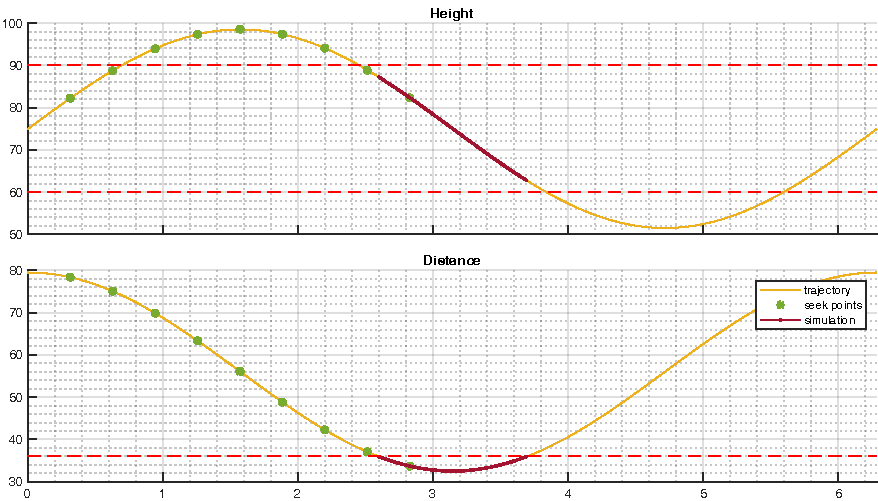
\includegraphics{heightdistance}
	\caption[Position eines Schneidenpunktes über Werkzeugwinkel]{Höhe im Werkstückkoordinatensystem und Entfernung vom Mittelpunkt des Werkstücks eines Schneidenpunktes aufgetragen über den Werkzeugwinkel}
	\label{fig:heightdistance}
\end{figure}

\begin{figure}
	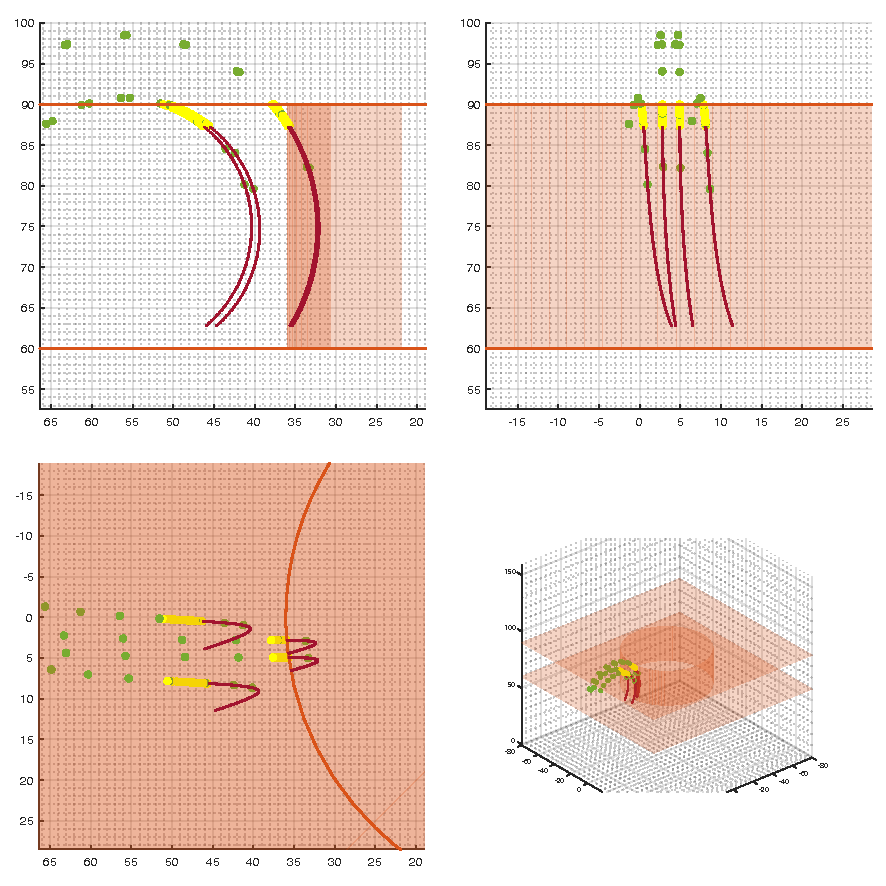
\includegraphics{3dview}
	\caption{3D Ansicht der Iterationsschritte bei der Findung der Startkonfiguration}
	\label{fig:3dview}
\end{figure}

\lstinputlisting[caption = {Findung der Startkonfiguration}, linerange=99-116,firstnumber=99, label={code:startkonfiguration}]{../ba/methods/vf1/vf1.m}

Die Abbildung \ref{fig:heightdistance} und \ref{fig:3dview} verdeutlichen das Vorgehen des in Codeausschnitt \ref{code:startkonfiguration} gezeigten iterativen Verfahren.
Die Panels der Abbildung \ref{fig:heightdistance} zeigen die Entwicklung von Koordinatenkomponenten eines Schneidenpunktes aufgetragen über den Drehwinkel des Werkzeugs, ausgehend von der Startkonfiguration.
Das obere der beiden Panels zeigt dabei die Höhe des Schneidenpunkte im Koordinatensystem des Werkstücks.
Der kontinuierliche Verlauf der Höhenkomponente ist dabei mit einer gelben Linie dargestellt.
Bei allen Konfigurationen des Werkzeugs wird die Höhe des Schneidenpunktes im Werkstückkoordinatensystem auf diesem Verlauf liegen.
Mit den rot strichlierten Linien ist die obere beziehungsweise untere Begrenzung der Werkstückausdehnung angedeutet.
Das untere Panel zeigt den Verlauf des Abstands des Schneidenpunktes von der Mittelachse des Werkstücks.
Hier ist ebenfalls der kontinuierliche Verlauf mit einer gelben Linie markiert.
Die äußere Begrenzung des Werkstücks wird durch eine rot strichlierte Linie dargestellt, die im Wert des Radius des Werkstücks verläuft.
Die Orte, für welche das Engagement des Werkzeugs geprüft wird, sind mit einem grünen Stern markiert.

In Abbildung \ref{fig:3dview} ist derselbe Vorgang dreidimensional dargestellt.
Dadurch wird die Position der seek-, Schnittkandidaten und Schnittpunkte im Raum ersichtlich.
Die äußeren Abmessungen des Bauteils sind durch ebene Flächen für die z-Ausdehnung und einen Zylinder für den Durchmesser des Bauteils markiert.
Man kann erkennen, dass der Algorithmus das Werkzeug so lange sprunghaft rotiert, bis mindestens ein Punkt der Schneide innerhalb der äußeren Bauteilabmessungen liegt.
Anschließend wird ausgehend von der obersten Schnittebene des Werkstücks nach einer validen Schnittkonfiguraiton gesucht, bis diese erreicht wird.
Der kontinuierliche Verlauf des Werkzeugs wird in dieser Darstellung nicht visualisiert um die Übersichtlichkeit nicht zu beeinträchtigen.

Man kann erkennen, dass bei diesem Verfahren die Rotation des Werkzeugs mit einer festen Schrittweite erfolgt, bevor Engagement überprüft wird.
Bei der letzten Prüfmarkierung sind erstmalig für diesen Schnitt die Engagement-Bedingungen erfüllt.
Die Position des geprüften Punktes liegt im Intervall der Höhenausdehnung und in der radialen Ausdehnung des Werkstücks.

Das Ziel des Findens der Startkonfiguration ist es, die Rotation des Werkzeuges zu finden, bei welcher das Werkzeug das Werkstück gerade berührt.
Der Seek liefert einen Werkzeugwinkel, welcher in der Nähe dieser Konfiguration liegt.
Durch Verkleinerung der Schrittweite beim Seeken kann die Lösungskonfiguration dieses Näherungsverfahrens näher an die tatsächliche Lösung geführt werden.
Allerdings muss die Berechnung des Engagements, also des Eingriffs der Schneide, für jeden Iterationsschritt erfolgen und sollte deswegen sehr günstig sein, somit wenig Rechenzeit in Anspruch nehmen.
Gleichzeitig muss ein Kompromiss zwischen der Größe der Schrittweite beim Seeken und der dafür notwendigen Rechenzeit gefunden werden.
Mit einem nachträglichen Schritt kann eine Lösungskonfiguration weit innerhalb des Werkstück-Envelopes geschickt ausgeglichen werden.

Sobald durch Iteration eine Konfiguration gefunden wurde, die als engaged gewertet wird, kann der so gefundene Winkel des Werkzeugs $B$ als Eingangswert $B_0$ für Gleichung \ref{eq:loesung} verwendet werden.
Neben dem Startwert $B_0$ sind für diese Funktion zur Lösung noch zwei Größen notwendig.

Zum einen muss die Höhe der Ebene in z, für die gelöst werden soll, gegeben sein.
Andererseits muss die Lösung der Funktion um den bereits zurück gelegten Winkel des Werkzeugs verschoben werden.

Dies geschieht über den Faktor $k$.
Wie in Abbildung \ref{fig:hobspindle_coord} zu sehen ist, liegt die Startposition des Werkzeugs auf der xz-Ebene im Koordinatensystem, oder ist zumindest in der Nähe.
Bis das Werkzeug bei einer Rotation das Werkstück erreicht, hat es in etwa eine halbe Umdrehung absolviert.
Diese halbe Umdrehung wird mit dem Summanden $k \cdot \pi$, mit $k=1$, berücksichtigt.
Die Lösung des Werkzeugwinkels muss im zweiten oder dritten Quadranten des Koordinatensystems liegen.
Der Lösungsbereich des Arkussinus ist $\left[-\frac{\pi}{2}, \frac{\pi}{2}\right]$.
Es muss also $\pi$ addiert werden um eine Lösung im dritten Quadranten, mit Wertebereich $\left[\frac{\pi}{2}, \frac{3\cdot \pi}{2}\right]$, zu erhalten.

Es ist noch nicht bekannt, auf welcher Ebene das Werkzeug das Werkstück initial berührt.
Auf dieser Ebene soll der Punkt des Werkzeugs für den gelöst wird liegen.
Der Wert der z-Koordinate dieser Ebene wird in Gleichung \ref{eq:loesung} als $z_{soll}$ bezeichnet.
Am Anfang der Simulation ist die geometrische Beziehung von Werkzeug und Werkstück nicht bekannt.
Die initiale Schnittebene kann aber geschickt durch ein iteratives Verfahren gefunden werden.
Gleichung \ref{eq:loesung} wird für einen Wert für $z_{soll}$ gelöst.
Anschließend wird für die Lösung $B$ geprüft, ob das Werkzeug in dieser Konfiguration engaged ist.
Ist dies nicht der Fall, wird für die Lösung die nächst tiefergelegene Ebene verwendet.
Das Werkzeug bewegt sich entlang seiner Rotation mit abfallender Höhe in z näher zur Achse des Werkstücks und kann so in Berührung kommen.
Für diese Ebene wird gelöst und wieder auf Engagement geprüft.

Das Resultat dieser Iteration wird in den Abbildungen \ref{fig:heightdistance} und \ref{fig:3dview} mit dem jeweilig ersten Punkt der dunkelroten Linien markiert.
Sie markieren die erste Konfiguration bei der sich mindestens ein Punkt der Schneide im Eingriff befindet.

Zwar muss so bei den iterativen Schritten ebenfalls wiederholt Engagement geprüft werden.
Allerdings kann die endgültige Lösung gespeichert und für die nächste Werkzeugumdrehung als Startebene verwendet werden.
Es kann bei gleichbleibendem Werkstückradius und geringem Vorschub in z-Richtung davon ausgegangen werden, dass die Kontaktebene bei der nächsten Umdrehung nahe der aktuellen liegt und somit nur wenige Iterationen notwendig sein werden.

Nach Finden einer Werkzeugkonfiguration die zu einem validen Schnitt führt, kann mit der Simulation des Schneidevorgangs begonnen werden.

\section{Berechnung des Werkzeugwinkels}
\label{c:berechnungwinkel}
Bei jeder Verschneidung der projizierten Werkzeugschneide mit der Werkstück Schnittebene ist die Berechnung des Werkzeugwinkels notwendig.

Die Eckpunkte der Schneide bewegen sich während der Rotation auf einer Kreisbahn um die Werkzeugachse.
Sie liegen dabei nicht zwangsläufig auf einer Ebene, die durch die Werkzeugachse geht oder parallel dazu ist.
Damit ist diese Schneidenebene nicht parallel zu den Schnittebenen des Werkstücks.
Das bedingt zwei grundsätzliche Probleme, die es zu lösen gilt.
Auf der einen Seite muss die Schneide des Werkzeugs auf die Werkstückebene projiziert werden, um die Verschneidungsberechnung durchführen zu können.
Die Projektion wird in Abschnitt \ref{c:schnitte} betrachtet.
Auf der anderen Seite gibt es für jeden Punkt der Schneide einen einzigartigen Winkel, den das Werkzeug annehmen muss, damit dieser Punkt auf einer Schnittebene des Werkstücks liegt.

Gelöst wird dieses Problem für jeden Punkt der Schneide durch Berechnung eines individuellen Winkels des Werkzeugs.
So werden alle Werkzeugwinkel gefunden, bei denen die Punkte auf der Zielschnittebene des Werkstücks liegt.
Dafür muss die Gleichung \ref{eq:loesung} gelöst werden.
Dabei handelt es sich um ein Fixpunktproblem.
Dem Fixpunktproblem zugrunde liegt eine Fixpunktgleichung der Form:
\begin{equation*}
	x = g(x)
\end{equation*}
Zur Lösung dieses Problems wird in \cite{Widmer1981} vorgeschlagen eine Fixpunktiteration durchzuführen.
Dabei wird die Gleichung umgeformt, sodass sie in folgender Form vorliegt:
\begin{equation*}
	x^{\left(n+1\right)} = g(x^{\,n}), \quad n = 0{,} 1{,} \dots
\end{equation*}
\begin{eqdscr}{$k$}
	\item[$n$] Iterationsindex
\end{eqdscr}
,,Für jede Wahl des Startpunktes $x^{(0)}$ konvergiert die Folge der Iterierten gegen [\dots]'' \cite{Widmer1981} die Lösung des Fixpunktproblems.
Da die iterative Methode fehlerbehaftet ist, ist es notwendig ein Abbruchkriterium einzuführen.
Dabei bietet sich die Änderung der Lösung zwischen Iterationen an.
Ist diese kleiner als ein definiert Wert, wird das Verfahren abgebrochen und die finale Lösung verwendet.
Diese Methode ist im Flussbild in dem Block ,,Iterationsschleife'' realisiert.

Entsprechend der Methode wird Gleichung \ref{eq:loesung} so angepasst, dass auf der rechten Seite statt $B$ die Lösung des vorhergehenden Iterationsschrittes $B_0$ verwendet wird.
\begin{equation}
	\label{eq:fixpunkt}
	B = k \cdot \pi - \phi_\wz + \arcsin{\left(\dfrac{Z - c - z_{soll} + B_0 \cdot{} \feed{Z}{Wz} + \sin(A) \cdot{} (Y + \yshift + B_0 \cdot{} \feed{Y}{Wz} - h_\wz)}
		{r_\wz \cdot{} \cos(A)}\right)}
\end{equation}
Diese Methode hat sich als sehr geeignet und effizient erwiesen.
So sind bei einer beispielhaften Simulation nur maximal zwei Iterationsschritte notwendig gewesen um das Abbruchkriterium von $1\cdot10^{-3}$ zu erreichen.
Der beim zweiten Iterationsschritt auftretende Fehler ist dabei überraschend gering, sodass lange nach einem Fehler in der Implementierung des Algorithmus gesucht wurde.
Der auftretende Fehler ist wie beschrieben definiert als die Änderung zwischen Eingangs- und Ausgangswert einer Iteration.
Bei dem beschriebenen Simulationsfall ist der Fehler nach der zweiten Iteration null.
Es wird vermutet, dass der Fehler kleiner ist als die Rechnengenauigkeit der CPU.

Die Methode bietet außerdem den Vorteil, dass als Startwert für die iterative Lösung des nächsten Werkzeugpunktes die letzte Lösung verwendet werden kann.
Das ist möglich, da bei geringem Abstand der Schnittebenen des Werkstücks auch die Lösungen nahe beieinander liegen müssen.

\lstinputlisting[caption = {Repräsentation der Fixpunktgleichungen als anonyme Funktionen}, linerange=79-91,firstnumber=79, label={code:anonfun}]{../ba/methods/vf1/vf1.m}

In dem Codeausschnitt \ref{code:anonfun} ist erkennbar, dass die Gleichung \ref{eq:fixpunkt} als anonyme Funktion definiert ist.
,,Eine anonyme Funktion ist eine Funktion, welche nicht in einer Programmdatei gespeichert ist.'' \cite{mwAnonFun}.
Sie wird stattdessen im Code definiert, und einer Variable des Datentyps Funktionshandle zugewiesen.
Sie steht damit auch nur dem Scope zur Verfügung in dem sie definiert wurde, und ist somit privat.

Diese Methode bietet hier den Vorteil, dass nur die funktionell relevanten Variablen als Argumente im Funktionsaufruf übergeben werden müssen.
Die Werte der übrigen Variablen, die sich nach Aufstellung des Simulationsfalles nicht mehr ändern, werden bei Definition der anonymen Funktion einmalig eingelesen und im Funktionshandle gespeichert.
Die funktionell relevanten Variablen sollen hier primäre Variablen, die übrigen sekundäre Variablen genannt werden.
Die anonyme Funktion hat keinen privaten Scope, verwendet also den Workspace der aufrufenden Instanz.
Es ist also wichtig dafür Sorge zu tragen, dass die sekundären Variablen innerhalb der anonymen Funktion gleich benannt sind wie außerhalb, um diese Funktionalität nutzen zu können.
Allerdings ist es wichtig zu erwähnen, dass der Wert der sekundären Variablen eingefroren ist nachdem sie in das Funktionshandle eingelesen wurden.
Ändert sich also der Wert einer Variable nach Definition der anonymen Funktion, wird diese Änderung nicht vererbt.

Gleichzeitig kann diese Operation vektorisiert ausgeführt werden.
Sie muss also nicht für jeden Punkt der Schneidengeomtrie einzeln ausgeführt werden, sondern die Eingangs- und Ausgangsgröße ist ein Zeilenvektor.
In diesem sind die Werkzeugwinkel für jeden Punkt der Schneide abgelegt.
Die Operationen werden elementweise ausgeführt und in einem gleichartig strukturiertem Vektor ausgegeben.
Diese Methode bietet gegenüber einer sukzessiven Berechnung einen großen Vorteil bei der Ausführungsgeschwindigkeit.

\lstinputlisting[caption = {Lösung der Fixpunktgleichung vor Durchführen eines Schnittes}, linerange=122-159,firstnumber=122, label={code:fixpunktloes}]{../ba/methods/vf1/vf1.m}

Der Codeausschnitt \ref{code:fixpunktloes} zeigt die Lösung der Fixpunktgleichung für jede diskrete Ebene des Werkstücks.
Nach jeder Lösung der Funktion in der Iterationsschleife wird überprüft, ob die erhaltenen Winkel real sind.
Das hat historische Gründe, da zu Beginn der Entwicklung nicht bedacht wurde, dass der Wertebereich des Arkussinus $\left[-1, 1\right]$ ist.
Wird der Funktion also vorgegeben den Werkzeugwinkel für eine Ebene zu berechnen, die kinematisch für das Werkzeug nicht mehr zu erreichen ist, wird der Wertebereich unterschritten.
Dieses Phänomen wurde verwendet, um das Ende des Schnittvorgangs zu erkennen.
Der Schnittvorgang ist beendet, wenn die Schneide des Werkzeugs nicht mehr im Eingriff ist.

Häufig ist der Schnitt jedoch beendet, bevor der tiefste Punkt der Werkzeugtrajektorie erreicht ist.
Um sich die Rechenzeit für Lösungsfindungen außerhalb des Werkstücks zu sparen wurde eine geschicktere Erkennung entwickelt.
Dabei wird wieder mit der Funktion \code{checkEng} geprüft, ob sich mindestens ein Werkzeugpunkt in der Hülle des Werkstücks befindet.
Sind alle Ecken der Schneide nicht mehr im Eingriff, wird angenommen, dass auch die Schneide nicht mehr im Eingriff ist.
Dabei wird zwar grundsätzlich der Fehler gemacht, dass ein Überlagerungsbereich von Werkzeug und Werkstück existieren kann, obwohl sich alle Eckpunkte der Schneide außerhalb der Schnittgeometrie des Werkstücks befinden.
Dieser wurde allerdings als so klein bewertet, dass er vernachlässigbar angenommen werden kann.

Diese Lösungsmethode wird dann in der Schnittschleife iterativ für jede diskrete Ebene durchgeführt, bis ein Austreten des Werkzeugs aus dem Werkstück erkannt wurde.
Dabei wird die Zielebene für die Lösung in absteigender Reihenfolge durch die vorhandenen diskreten Ebenen des Werkstücks gewählt.

\section{Durchführung der Schnitte}
\label{c:schnitte}
Nach Berechnung der Lösungswinkel wird als nächstes der Schnitt des Werkzeugs ausgeführt.

Zu Beginn der Beschreibung der Schnittsimulation soll erklärt werden, wie in der Simulation ein Schnitt berechnet wird.
Werkzeug und Werkstück werden als Polygone repräsentiert, die in \matlab als Objekt der Klasse polyshape dargestellt werden.
Polyshape Objekte haben Methoden, die es erlauben Verschneidungsoperationen durchzuführen.
Dabei wird von einem polyshap Objekte die Geomtrie abgezogen, die von dem anderen Polygon überlagert wird.
\begin{figure}
	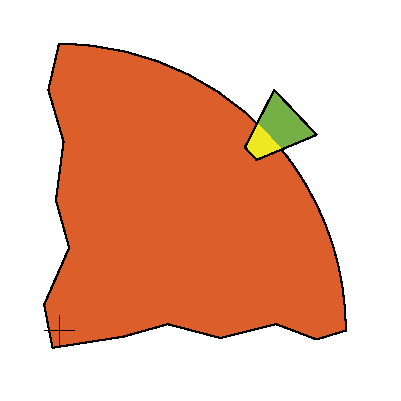
\includegraphics{uberlagerung}
	\caption{Überlagerungsbereich von zwei Polygonen}
	\label{fig:uberlagerung}
\end{figure}

In Abbildung \ref{fig:uberlagerung} ist eine solche Überlagerungssituation dargestellt.
Das Werkzeug wird als grünes Polygon gezeigt, eine Schnittebene des Werkstücks als orangenes Polygon.
Der Abstand der Polygoneckpunkte der Werkzeugschnitte ist dabei sehr niedrig gewählt um den Sehnenfehler zu minimieren.

Die Sehne einer Raumkurve ist die gerade Verbindung von zwei Punkten entlang der Kurve.
Sie kann verwendet werden, um den Verlauf der Raumkurve unbekannter mathematischer Entstehung geschickt anzunähern.
Ist die Raumkurve gekrümmt, existiert über den Verlauf der Sehne ein Abstand zwischen Kurve und Gerade.
Das Maximum dieses Abstands ist definiert als der Sehnenfehler.
Dieser kann verringert werden, wenn der Abstand der Punkte auf der Raumkurve verringert wird.
Durch eine hohe Anzahl von Eckpunkten bei einem Polygon werden die Sehnen kürzer, der Sehnenfehler sinkt und die Rundheit des Polygons steigt.

Zusätzlich wurde bei der Diskretisierung des Werkstückzylinders in Schnittebenen die Position der Eckpunkte abwechselnd um den halben Abstand der Sehnenpunkte verschoben.
Damit kann der mittlere Abstand der diskreten Punkte auf der Oberfläche des Zylinders verringert werden.
So entstehen bei der Vernetzung des Simulationsergebnisses auf der unbearbeiteten Oberfläche des Werkstückes nicht-rechtwinkelige Dreiecke.
Derartige Dreiecke sind für die gängige Vernetzungsalgorithmen besser geeignet als rechtwinkelige.

Es wurden keine Versuche angestellt die Rundheit der Schnittgeometrien zu berechnen und die Simulationsgenauigkeit in Abhängigkeit davon zu bewerten.
Auch gilt es noch zu untersuchen, welchen Einfluss die Anzahl der Eckpunkte bei der Diskretisierung auf die Simulationsgeschwindigkeit hat, da dieser als gering vermutet wurde.

Die in Abbildung \ref{fig:uberlagerung} gelb dargestellte Fläche ist der Überlagerungsbereich von Werkzeug- und Werkstückoperation.
Dieser überlagerte Bereich wird bei der Simulation der Schnittoperation von dem Werkstückpolygon abgezogen.

\lstinputlisting[caption = {Verschneidung der überlagerten Polygonbereiche}, linerange=161-178,firstnumber=161, label={code:uberlagerung}]{../ba/methods/vf1/vf1.m}

Die in dem Codeausschnitt \ref{code:uberlagerung} gezeigte Operation wird in der Simulation durchgeführt, nachdem alle Winkel berechnet wurden, bei denen die Eckpunkte der Schneide auf einer Schnittebene liegen.
Um eine Überlagerung von Werkstück und Schneide berechnen zu können, müssen die beiden Geometrien koplanar sein.
Wie in Abschnitt \ref{c:berechnungwinkel} erwähnt, muss dazu die Schneide auf die Werkstückschnittebene projiziert werden.
Diese Operation wird für jeden Punkt einzeln durchgeführt.
Für die Projektion müssen die Koordinaten der Schneide im Koordinatensystem des Werkstücks vorliegen.
Dazu wird die vektorielle Gleichung \ref{eq:koordgleichung} ausmultipliziert.
Man erhält eine Gleichung je Koordinatenachse, die maßgeblich von dem Werkzeugwinkel abhängt.
Ähnlich zu dem Vorgehen die Gleichung \ref{eq:fixpunkt} wird sie als anonyme Funktion definiert.
Die Konstanten werden ebenfalls bei Erzeugung eingelesen und in das Handle gespeichert.
Auch Gleichung \ref{eq:koordgleichung} könnte vektoriell verwendet werden.
Dafür müssten die Dimensionen der Matrix der Schneidenkoordinaten und der Werkzeugwinkel aber senkrecht aufeinander stehen, die Lösung wäre dann ein Tensor.
Jede Matrix des Tensors wäre dann die transformierten Koordinaten bei einem Winkel.

Der Aufbau von Koordinatenmatrizen in der Simulation unterscheidet zwischen Punktewolken und zeitvarianten Punkten.
Eine Punktewolke ist ein Menge von Punkten die sich im vorliegenden Fall dadurch auszeichnen in einer zeitinvariant festen räumlichen Anordnung zueinander zu stehen.
Sie wird beschrieben durch eine Matrix aus Spaltenvektoren der Koordinatenkomponenten eines Punktes.
Diese Matrix ist zweidimensional.

Im Gegensatz dazu sind zeitvariante Punkte eine Menge von Punkten, die ausgehend von einem oder mehreren Punkten in Schritten von einer Start- zu einer Zielanordnung schrittweise transformiert werden.
Zu jedem Zeitschritt werden diese Punkte in einer Punktewolkenmatrix abgelegt.
So ergibt sich ein Tensor von Punktewolken zu verschiedenen Zeiten.
Die Abhängigkeit von der Zeit ist nur formell, weil angenommen wird, dass bei der Bewegung eines physikalischen Systems Zeit vergeht.
Grundsätzlich ist die vorliegende Simulation nicht zeitabhängig.
Die verschiedenen Werkzeugwinkel je Schnittebene wären dann genau solche Transformationsschritte.

In der vorliegenden Implementierung wird die Berechnung der Schneidenkoordinaten im Werkzeugkoordinatensystem allerdings noch in einer Schleife über die Werkzeugwinkel ausgeführt.
Die gefundenen Koordinaten werden in das Koordinatenfeld des Polyshape Objektes der Schneide eingetragen.
Danach kann die Verschneidung des Überlagerungsbereiches von Werkzeug und Werkstück erfolgen.
Dabei wird für jeden Vertice der Werkzeugschnittgeometrie nachverfolgt, wie dieser zustande gekommen ist.
Dabei gibt es drei Ursprungsmöglichkeiten.
Der Punkt kann bei Erzeugung des Schnittebenenpolygons erzeugt worden sein, also originaler Bestandteil der Geometrie sein.
Er kann entstanden sein durch die Verschneidung einer Werkzeugkante mit einer Werkstückkante.
Am Schnittpunkt dieser Kanten wird ein Punkt erzeugt, der in die Menge der Vertices des Werkstückpolygons aufgenommen wird.
Außerdem werden bei der Verschneidung Punkte des Werkzeugpolygons, welche innerhalb des Werkstückpolygons liegen, in die Menge der Werkstückvertices aufgenommen.

Die Verschneidungsmethode der Polyshape Objekte gibt diese Klassifikation für jeden Schritt zurück.
Allerdings ist der Methode nicht bekannt, welchen Ursprung ein Punkt vor der Verschneidung vor der Schnittoperation hatte.
Dafür werden aus der zurückgegebenen Klassifikation ausschließlich die Punkte herausgefiltert, die bei der durchgeführten Schnittoperation entstanden sind.
Nur für diese Punkte wird die Klassifikation in den Klassifikationsvektor übernommen.

\section{Schnittende}
Ein Schnitt ist die Menge direkt nacheinander stattfindende Engagementkonfiguration der Werkzeugschneide.
Wir beschrieben beginnt der Schnitt mit der ersten gefundenen Konfiguration des Werkzeugs bei der eine Überlagerung stattfindet.
Der Schnitt ist beendet, wenn die Schneide des Werkzeugs nach einer Überlagerungskonfiguration den ersten Iterationsschritt nicht mehr engaged ist.
Dieser Zustand wird mit der beschriebenen Methode erkannt.

\lstinputlisting[caption = {Operation bei Erreichen des Schnittendes}, linerange=180-192,firstnumber=180, label={code:schnittende}]{../ba/methods/vf1/vf1.m}

Ist bei dem Codeausschnitt \ref{code:schnittende} das Schnittende erreicht, wird nur der größte gefundene Werkzeugwinkel behalten.
Es kann davon ausgegangen werden, dass die Schneide einen Anteil einer Umdrehung zurücklegt, bis sie wieder in Eingriff geraten kann.
Die Größe des Winkels hängt von der Anordnung von Werkzeug und Werkstück ab.
Eine zuverlässige Annahme ist eine halbe Umdrehung.
Der Winkel einer halben Umdrehung, $\pi$, kann also auf den größten Werkzeugwinkel addiert werden und als neuer Startpunkt der Seekoperation verwendet werden.

Der Sprung des Werkzeugs kann alternativ auf den bei der Findung der Startkonfiguration gefundenen Winkel bezogen werden.
Die Geschwindigkeit der Werkzeugrotation ist im Verhältnis zu den Vorschubgeschwindigkeiten sehr hoch.
Eine Annahme, dass der Winkel bei initialem Engagement des nächsten Schnittes ungefähr dem Winkel des vorherigen Schnittes entspricht, ist daher zulässig.
Ist der Vorschub der X-Achse ungleich null, verändert sich der Achsabstand von Werkzeug und Werkstück.
Das hat einen Einfluss auf den Winkel bei dem das Werkstück in den Eingriff gerät.
Die während einer Werkzeugumdrehung zurückgelegten Strecke der X-Achse wird aber gering sein.
Der Engagementwinkel wird daher in der Nähe des zuletzt gefundenen liegen.
Bei Anwendung dieses Vorgehens entfällt die Notwendigkeit des Seekens nach dem ersten Schnitt.
Wie bei dem initialen Seeken kann ein Eintritt der Schneide in das Envelope des Werkstücks ist mit der in Abschnitt \ref{c:startkonfig} Methode kompensiert werden.

Mit der gleichen Begründung kann angenommen werden, dass die oberste Schittebene des folgenden Schnittes in der Nähe der letzten obersten Schnittebene liegt.
Um mit Sicherheit alle Lösungen zu betrachten, wird die Suche nach validen Schnittebene oberhalb der letzten Startebene gestartet.
Damit sind die Vorschübe der X-Achse und Z-Achse abgedeckt, die Einfluss auf die oberste Schnittebene haben können.

Die Schneide wird sich bei der nächsten Umdrehung in der nächsten Periode des Lösungsbereichs der Gleichung \ref{eq:fixpunkt} befinden.
Die Periode dieses Lösungsbereich ist eine volle Werkzeugumdrehung.
Zu dem Faktor $k$ muss somit zwei addiert werden, damit der Lösung ein Inkrement von $2 \pi$ aufgeprägt wird.

Abschließend wird geprüft, ob das Stop Criterion der Simulation erreicht.
Im aktuellen Stand ist vorgesehen, das Ende der Simulation darüber zu steuern, welchen Winkel das Werkstück gelegt hat.
Dieser wird mit der Definitionsgleichung \ref{eq:wrkstwinkel} der Werkstückrotation in Abhängigkeit des Werkstückwinkels berechnet.

Es ist ebenfalls denkbar, die Bearbeitung eines einzelnen Zahnzwischenraums zu betrachten.
Dabei müsste nach Vollendung eines Schnittes dem Werkzeugwinkel $B$ der Winkel addiert werden, den das Werkzeug nach einem Umlauf um das Werkstück hat.
Das Werkzeug vollzieht je Zahnzwischenraum eine volle Umdrehung.
Der übersprungene Winkel ist folglich
\begin{equation*}
	B_{"ubersprungen} = \left(n_{Z"ahne} -1 \right) \cdot 2 \pi
\end{equation*}
\begin{eqdscr}{$B_{"ubersprungen}$}
	\item[$B_{"ubersprungen}$] übersprungener Winkel des Werkzeugs
	\item[$n_{Z"ahne}$] Zähnezahl des Werkstücks
\end{eqdscr}
Bei dieser Simulationsmethodik bietet sich dann ein Zähler der durchgeführten Schritte an um die Simulation zu stoppen.

\section{Plotten}
\begin{figure}
	\includegraphics[width=\textwidth,keepaspectratio]{pointcloud}
	\caption{Ausgegebene Punktewolke}
	\label{fig:pointcloud}
\end{figure}

Die Abbildung \ref{fig:pointcloud} zeigt die dreidimensionale Ausgabe der Punktewolke des Simulationsergebnisses.
Diese Darstellung wird während der Simulation in Echtzeit ausgegeben und zeigt somit immer den aktuellen Stand der Simulation.

Die Herausforderung bei der grafischen Ausgabe war es einen möglichst geringen Einfluss auf die Ausführungsgeschwindigkeit der Simulation zu nehmen.
Darüber hinaus ist es wünschenswert den Simulationscode möglichst gut lesbar zu erhalten, um die Fehlersuche bei der Entwicklung zu vereinfachen.
Es wurde daher entschieden, Simulation und Ausgabe zu trennen.
Eine geschickte Möglichkeit diese Trennung zu erreichen ist eine Klasse zu entwickeln und der Simulation so die gewünschte Funktionalität in der grafischen Ausgabe bereitzustellen.
Eine Klasse ist ein Konzept der Objektorientierten Programmierung.
Sie bieten die Möglichkeit Daten und Funktionen in einer Struktur zu vereinen.

Bei Erzeugung eines Objekts der \code{plotSimulation}-Klasse wird die grafische Ausgabe eingerichtet und relevante Werte des Simulationsfalles eingelesen.
Diese werden in dem Objekt gespeichert und stehen ohne Zugriff auf den Basis-Workspace zur Verfügung.
Die Handles der Ausgabefenster, der Achsen- und der Linienobjekte werden ebenfalls in dem Objekt gespeichert.
Auf sie kann zu einem späteren Zeitpunkt zu gegriffen werden, um die Objekte anzusprechen.

Eine wichtige Komponente der \code{plotSimulation}-Klasse ist das \code{timer}-Objekt mit dem Funktionen in definierten Intervallen ausgeführt werden können.
So können die teuren Ausgaberoutinen mit einem festen Intervall ausgeführt werden statt bei Erreichen eines Zustands bei der Ausführung der Simulation.
Diese Funktionalität ist realisiert, in dem die Simulationsschleife dem Ausgabe-Objekt Werte bereitstellt welche aber nicht unverzüglich grafisch ausgegeben werden.
Stattdessen werden die Daten in dafür vorgesehene Felder des Objekts geschrieben und erst im nächsten Intervall geplottet.

In \matlab existieren Plottingroutinen die für diese Architektur gedacht sind.
Sie haben einen Cache, in den konstant Daten geschrieben werden können.
Sobald ein Aufruf der Ausgabefunktion erfolgt, werden die Daten in die grafische Ausgabe geplottet.

Im aktuellen Stand kann so eine Ausgabefrequenz von $0{,}5 \si{\hertz}$ erreicht werden die ungefähr ein Drittel der Ausführungszeit der Simulation benötigt.
Der hohe Aufwand der notwendig ist um in \matlab dieses Ergebnis zu erreichen zeigt, dass eine externe oder nachträgliche Visualisierung der Simulation notwendig ist.
Die aktuell grafisch zur Verfügung gestellten Information sind aber sehr hilfreich bei der Entwicklung der Routinen, weswegen nur schwer auf sie verzichtet werden könnte.
Es ist sehr wenig Aufwand kann die Ausführungszeit der Simulation verbessert werden in dem die Aufrufe zu dem Plot-Objekt ausgelassen werden.

Die Abbildungen \ref{fig:heightdistance}, \ref{fig:3dview}, \ref{fig:uberlagerung} und \ref{fig:pointcloud} werden während der Simulation in Echtzeit aktualisiert.
Sie haben sich trotz dem negativen Einfluss auf die Ausführungsdauer der Simulation als äußerst hilfreich erwiesen um den Fortschritt und das Verhalten der Simulation zu überwachen.
So konnte zum Beispiel mit Hilfe von Abbildung \ref{fig:heightdistance} erkannt werden, dass ein Abbruchkriterium für jeden Schnitt notwendig ist.
Ohne dieses Abbruchkriterium versucht der Algorithmus nach Erreichen des tiefsten Punktes auf der Trajektorie der Schneideneckpunkte eine noch tiefere Schnittebene des Werkstücks zu erreichen.
Dies war die Ursache, für die während der Entwicklung festgestellte imaginäre Lösung der Gleichung \ref{eq:fixpunkt}.
